%!TEX root = ../masters_thesis.tex

% ==============================================================================
  -> Managing Vagueness, Uncertainty and Granularity in Spatial Information Systems (VUG)
  %http://www.geos.ed.ac.uk/~gisteac/gis_book_abridged/files/ch13.pdf
  %http://link.springer.com/chapter/10.1007%2F978-3-642-14755-5_1
  %http://support.esri.com/en/knowledgebase/GISDictionary/term/uncertainty
  %http://www.geog.ucsb.edu/~kclarke/G176B/Lecture07.ppt
  -> Karl Grasser (Diss. Santa Barbara)
  -> Fuzzy, Imprecice,
  proabilities vs. possibilities

big problem: why? intention and motivation of author? hard to find out...
voice and perspective
medieval maps: natural landmarks as border points => inaccurate and imprecise
perspective: who is making the map? (illiterates?)
different names:
  US Civil War (North) vs.
  WWI (West) vs. Germanic War (Russia)
  WWII (West) vs. Great Fatherland War (Russia)

accepted uncertainty: date != exact timepoint, only D.M.Y
                      location != exact location, only name of place

\cite[chapter 2, p. 51]{solana2014spatio}

think about how to represent historical knowledge in geographic context
degree of certainty -> ironically: that has to be exact as well in a database table
=> reason: careful conclusions from historical maps

different states of boundaries: draft -> proposal -> dispute ->
% \cite Wachowitz 1998

% ==============================================================================


\chapter{Uncertainty} % (fold)
\label{cha:uncertainty}

Every aspect of the concept (chapter \ref{cha:concept}) and the development (chapter \ref{cha:development}) of this work is based on the prerequisite of full certainty of the data. That means both the Historical-Geographic Operations and the Hivent-Based Spatio-Temporal Data Model assume that the dates of the historical events, the names and territories of the historical and current areas and the historical relations between events and areas are accurate and reasonably precise (definitions see \ref{sec:types_of_uncertainty}).

However, this assumption is far from valid. In historical research, uncertainty is one of the major problems (see \ref{sub:history}) a historian has to deal with on a daily basis: sources, even primary sources, can be biased towards the author of the source, information can be imprecise or even inaccurate and information can be conflicting with other sources. This chapter explains problems with uncertainty in the domain of development of countries in time and space and develops approaches to deal with these problems.


% ==============================================================================
\section{Definition of a Country} % (fold)
\label{sec:definition_of_a_country}

The problem begins with the definition of a term that almost everybody in the world is familiar with: a ``country''. Since countries are the domain of this historical geographic information system, it must be possible to decide for each current and historic territorial entity in the world if it is or was a country or not. Therefore a clear and non-conflicting definition of a country is necessary. However, this is impossible to do.

The Oxford Dictionary definition of a country reads as follows:
\begin{quote}
  ``The \emph{territory} of a \emph{nation}; a \emph{region} constituting an \emph{independent state}, or a region, province, etc., which was once independent and is still distinct in institutions, language, etc.''
  \footnote{\textit{country, n. and adj}, Oxford English Dictionary, URL: \url{http://www.oed.com/view/Entry/43085?}, last access: 2016-04-25}
\end{quote}

This definition includes many different concepts and terms: the territory or region that the country is on, a nation or state, a population and a culture of the territory in terms of institutions or languages. While nation and state are commonly used as synonyms for countries, their meaning varies from case to case, as it will be examined in this section.

To understand what a country really is, the United Nations as an intergovernmental organisation are a valuable source. It was found after World War II (October 1945) and promotes international peace keeping, security, protection of human rights or humanitarian aid to all its member states which should coincide with all the countries in the world. The committee currently has 193 full member states and two permanent obervers: The Holy See (Vatican City) and the State of Palestine \cite{UNmembers}. But these 195 members in total do not cover all places in the world -- and also a membership in the United Nations does not mean that the question of statehood can simply be answered.

% ------------------------------------------------------------------------------
\subsection{Special Cases} % (fold)
\label{sub:special_cases}

Examining the list of the UN member states yields several interesting observations and special cases, which can be classified by their membership status in the United Nations and their degree of international recognition.


\paragraph{UN observer states} % (fold)
\label{par:un_observer_states}

The \emph{Holy See} is the juridcal and spiritual entity representing the territory of Vatican City. It is a fully recognized and sovereign state but is not a full member of the UN, because it has never applied for it. It is the by far smallest sovereign state in the world (0.44 m²), is an enclave inside the city of Rome with a population of only 800 people, including 30 women \cite{VaticanPopulation}.

The \emph{State of Palestine} has a population of 4.8 million people \cite[as of 2016]{PalestinePopulation} and is also an UN observer state. However, it is totally different in terms of sovereignty: While it consists of the territories of the West Bank, East Jerusalem and the Gaza Strip, their borders were drawn in the 1949 Green Line Armistice Agreement but were never intended to be used as international boundaries \cite{PalestineTerritory}. Since then, the ongoing and complex conflict with the State of Israel lead to a difficult situations regarding the sovereignty over the territories. Therefore, the state has no clearly defined territoy. Moreover, while 114 states officially recognize the Palestinian state, almost all current main economic powers do not, including the Canada, France, Germany, Italy, the United Kingdom and the United States. None of them even voted in favor of Palestine receiving an observing status in the UN \cite{PalestineUN}. That means, unlike the Holy See, Palestine is not a fully sovereign and recognized state.

% paragraph un_observer_states (end)

\paragraph{UN non-members with limited recognition} % (fold)
\label{par:un_non_members_with_limited_recognition}

\emph{Kosovo} is a state Europe and and declared independence from Serbia in 2008. It has a clearly defined territory and a permanent population and is recognized by 111 UN member states. In order for Kosovo to become a full member of the United Nations, all permanent members of the security council (United Kingdom, France, Russia, China and the United States) must agree. But since Russia and China strongly support the territorial integrity of Serbia, they would veto Kosovos membership in the United Nations. Therefore, Kosovo is not even an observer state of the United Nations, although having about the same degree of international recognition as Palestine \cite{KosovoThanksYou}.

The status of Taiwan is a very complicated issue. An overgeneralized description of the problem, which involves two territories and two political entities, is: There is the \emph{People's Republic as China} (commonly known as China), with full control over mainland China, and the \emph{Republic of China}, governing the island of Taiwan. However, both political entities claim each others land. That means, there are two states claiming the exact same territory. But, since 1971 the People's Republic of China is the representative of whole China in the United Nations, including the island of Taiwan. Because it is part of the Security Council, it successfully vetos membership requests of the Republic of China. Therefore, it can not be a member of the United Nations, although it operates like an independend country by international standards: They have an own jurisdiction, issue own passports and have unofficial diplomatic relations to most countries in the world. But officially, only 22 member states of the United Nations uphold diplomatic relations to Taiwan \cite{TaiwanRecognition}. To all of these states the People's Republic of China does not have any diplomatic relations, which makes also them an only partially recognized state.

There are other non-member states of the United Nations which have not yet gained broad international recognition: the Sahrawi Arab Democratic Republic (recognized by 84 UN member states \cite{WesternSaharaRecognition}), Abkhazia (6 \cite{AbkhaziaRecognition}), South Ossetia (5 \cite{SouthOssetiaRecognition}), the Turkish Republic of Northern Cyprus (1 \cite{NorthernCyprusRecognition}), Nagorno-Karabakh Republic (0 \cite{NagornoRecognition}), Transnistria (0 \cite{TransnistriaRecognition}) and Somaliland (0 \cite{SomalilandRecognition}).

% paragraph un_non_members_with_limited_recognition (end)

\paragraph{UN members with limited recognition} % (fold)
\label{par:un_members_with_limited_recognition}

In addition to the Republic of China, there are five other member states of the United Nations that are not fully recognized by all other UN members: Armenia (not recognized by Pakistan \cite{ArmeniaRecognition}), the Republic of Cyprus (not recognized by Turkey \cite{CyprusRecognition}), North and South Korea (officially Democratic People's Republic of Korea and Republic of Korea, mutual non-recognition \cite{KoreaRecognition}) and the State of Israel, which 32 UN member states do not recognize \cite{IsraelRecognition}.

% paragraph un_members_with_limited_recognition (end)

\paragraph{Special Territories} % (fold)
\label{par:special_territories}

Additionally to countries gaining for international recognition there are territories belonging to fully sovereign countries with a varying degree of sovereignty. For example Greenland is an autonomous country within the Kingdom of Denmark, but not a  sovereign state and therefore not a member of the United Nations. The same applies to the Faroer Islands (part of Denmark) and numerous overseas territories of the United Kingdom, the French Republic and the Kingdom of the Netherlands in the Carribean, the Indian Ocean or the Southern Pacific Ocean. Moreover, there are five quasi-independent countries in a so called \emph{Free Association}: Niue and Cook Islands are associated to New Zealand and not part of the United Nations. The Marshall Islands, the Federated States of Micronesia and Palau are associated to United States, but in contrast are full UN members \cite{SpecialTerritories}.

% TODO?
% example United Kingdom:  country?
% difference clear: geography             politics
%                   British Isles         United Kingdom of Great Britain and NI
%                     Great Britain         Scotland, England, Wales, Northern Ireland (province)
%                     Ireland             Republic of Ireland
%                     Shetland Islands
%                     Isle of Men
%                     ...

% Scotland, England and Wales are countries, but not sovereign states, Northern Ireland is a province and not a country. The UK is a constituent country, just like the Kingdom of the Netherlands and the Kingdom of Denmark.

% paragraph special_territories (end)

This incomplete and simplified list of special cases manifests the big problem that is associated with the terms ``country'', ``state'' or ``nations'': There is neither a \emph{de jure} consistent definition nor a \emph{de facto} consistent usage of these terms. Everything breaks down to two different concepts:


% subsection special_cases (end)

% ------------------------------------------------------------------------------
\subsection{Declaratory vs. Constituitive Theory} % (fold)
\label{sub:declaratory_vs_constituitive_theory}

The declaratory theory, established in the Montevideo Convention 1933 \cite{MontevideoConvention}, gives each entity the right to declare a state if it matches all of the four requirements:
\begin{compactenum}
  \item a clearly defined territory
  \item a permanent population
  \item a political representation / government
  \item the \emph{capacity} to enter diplomatic relations
\end{compactenum}

These four requirements make sure that a state can exist physically and politically. However, it is worth noticing that this definition does not include any actual diplomatic relations to other states, but only the capacity to enter them. Therefore the existance of a state is independent from its recognition by other states. In other words: ``A country is a country when it thinks it is a country.''

In contrast, the constituitive theory requires exactly that: A state can only be considered as such if it is recognized by other states. However, it is not defined anywhere by how many other states \cite{StateTheory}. In short: ``A country is a country when other countries think that country is a country.'' \cite{greyCountries}

\begin{figure}[ht]
  \centering
  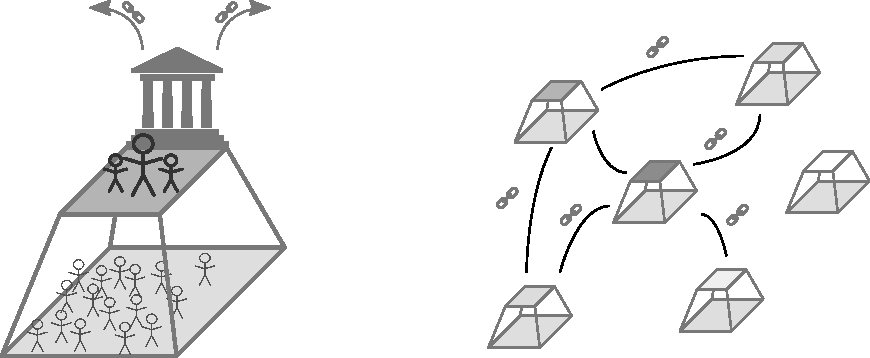
\includegraphics[width = 0.8\textwidth]{graphics/uncertainty/decl_const_theory}
  \caption{The Declaratory Theory (left) and the Constituitive Theory (right) of Statehood}
  \label{fig:declaratory_constituitive_theory}
\end{figure}

Both theories have advantages and disadvantages, but the two main problems are:
\begin{enumerate}
  \item Following the declarative theory, countries are self-classifying and potentially conflicting entities. The application of this measure would grant Kosovo, the Republic of China, Abkhazia or the Sarhawi Arab Democratic Republic full statehood. However, since their territories are contested, this would lead to overlapping territories with Serbia, China, Georgia and Morocco, which is impossible.
  \item There is no superior organization that can judge if a country is a country or not. Even the United Nations fail to do so, because their membership requirements prevent states like Kosovo or the Republic of China from becoming full members. They also have no power to rule out problems regarding the independence of Transnistria or Somaliland.
\end{enumerate}

Therefore it is impossible to objectivly classify an area as a country or not: nobody can say if Kosovo, the State of Palestine or Niue are countries or not. These theories have been introduced in the previous 80 years. For the time before that, a conflict-free decision of what is country is not just impossible, but also not justifyable because of a lack of jurisdiction.

That means, an historical geographic information system with the goal to visualize the development of the countries on Earth in time and space inevitably deals with uncertain information that certain parties see as wrong. Its data model can not perfectly fit self-classifying data and can not rely on an objective data source. The system has to contain approaches that deal with this problem.

% subsection declaratory_vs_constituitive_theory (end)

% section definition_of_a_country (end)


% ==============================================================================
\section{Types of Uncertainty} % (fold)
\label{sec:types_of_uncertainty}

In order to understand different types of uncertainty it is important to understand the concepts of \emph{disagreement}, \emph{precision} and \emph{accuracy}.

The model in an information system tries to resemble the real world as good as possible and necessary -- in this case the history of countries. If there is already a conflict in the real world, e.g. the Kasmir region which is claimed by both India and Pakistan as part of their territory, then this is a \emph{disagreement} which also has to be proberly modeled as such in the system.

The better a model simulates the reality, the more \emph{accurate} or correct it is. That means, the closer it gets to the target, the higher is the accuracy. \emph{Precision} or exactness describes how similar the results are compared to each other, independent from the distance to the target. That means a precise model gets the same results over and over again (see figure \ref{fig:accuracy_precision}).

\begin{figure}[ht]
  \centering
  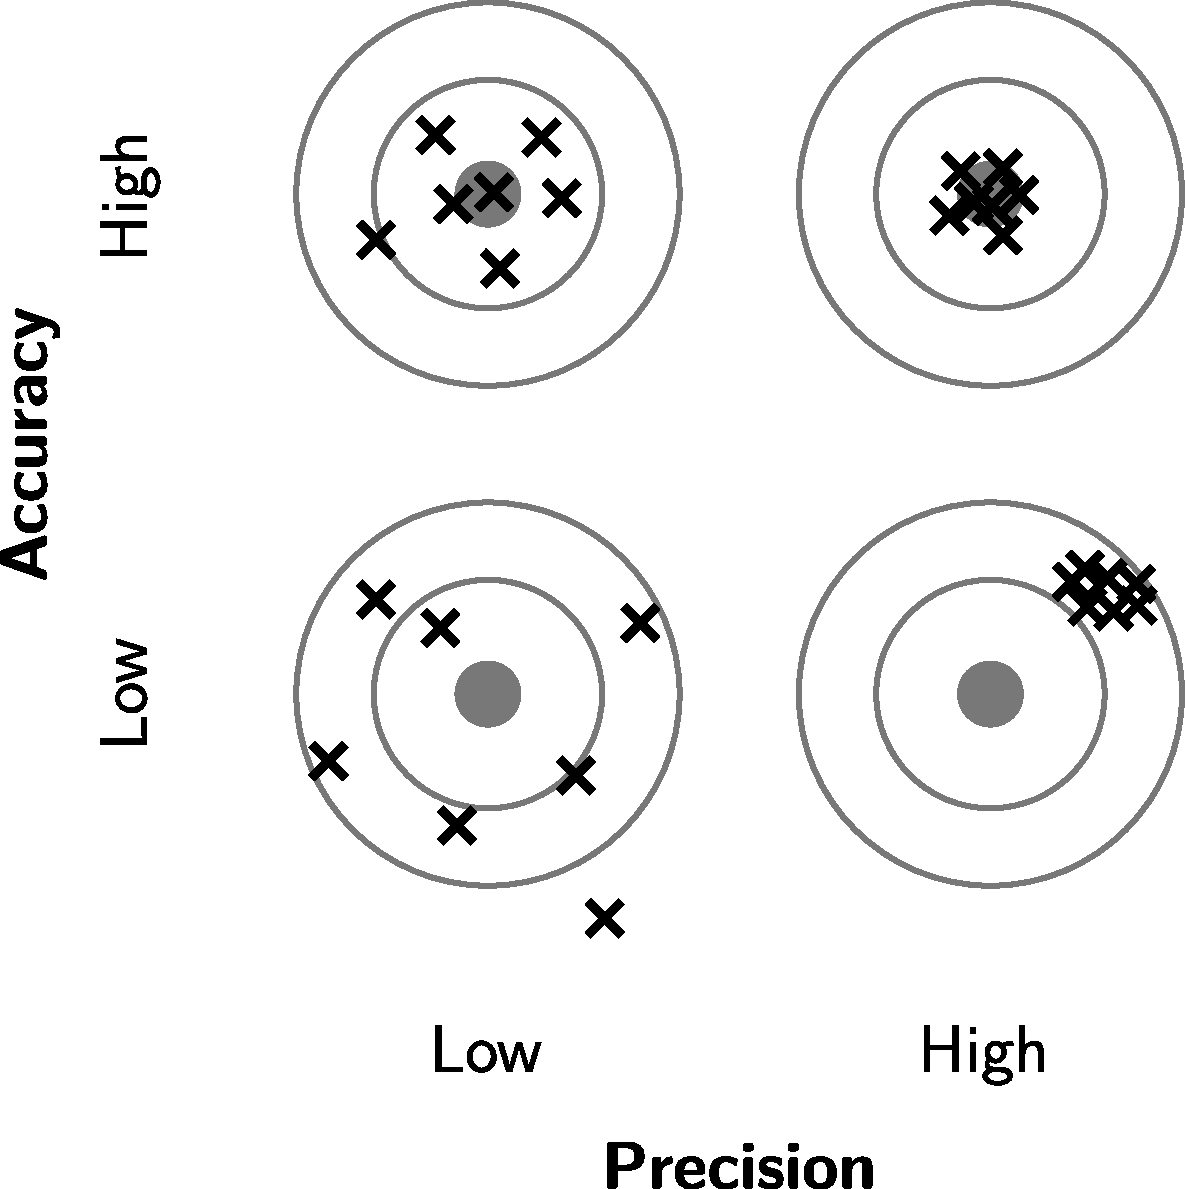
\includegraphics[width = 0.35\textwidth]{graphics/uncertainty/accuracy_precision}
  \caption{The difference between accuracy and precision}
  \label{fig:accuracy_precision}
\end{figure}

If the border between the Principalities of Transsylvania and Wallachia is deducted from an historical map of 1600, the course of the border is is inaccurate to a certain degree, because the map does not show the real world correctly. However, it can be modelled in the system very precisely, because the coordinates of the border points are stored as floating point numbers in the data model. In contrast, there is currently no agreement upon territory of Palestine, although the different versions can be modelled very precisely. In order for the model to also be accurate in this case, it would need to support contested territories.

Hereafter the current data model introduced in section \ref{cha:development}
% TODO: reference to actual section with the data model
is evaluated in terms of accuracy and precision.


\paragraph{Hivents} % (fold)
\label{par:evaluation_hivents}

The model for historically significant happenings contains only the following meta information: name, date and location of the event. This has several shortcomings in terms of precision:

The name of an historical event can have different versions: a long, official version and a short common version. The commonly known ``Treaty of Versailles'' (1919) is officially called the ``Treaty of Peace between the Allied and Associated Powers and Germany''. Also the name is different in other languages affected by the treaty. Additionally, there can be different versions of the name from different perspectives, even within the same language, e.g. the ``American Civil War'' as it is known today was alternatively called ``War Between the States'', ``War for Southern Independence'' or ``War of Northern Aggression'' depending on the perspective.
The ~\texttt{Hivent}~ model does not account for different languages and versions and is therefore not very precise.

The ~\texttt{Hivent.date}~ is supposed to represent the temporal dimension of an historical event. While an historical change itself is discrete and happens at exactly one time point, the historical event yielding this change might not. The ``Congress of Vienna'' which reordered the empires on the European mainland was one of the main historical events in modern European history. While the changes of the congress came into effect on 9. June 1815, the congress itself took place in Vienna from September 1814 until June 1815 which is also a timespan of interest. Another phenomenon becomes apparent in the ``Convention for the Extension of Hong Kong Territory'' (1898) which had a predefined length of 99 years. The treaty therefore has two dates in which historical changes happened: the date the treaty came into effect (Hong Kong becomes part of the United Kingdom) and the date it stopped being in effect (Hong Kong is handed over to China). Other interesting aspects are different calendar systems used in different parts of the world throughout history: the October Revolution in Russia (1917) happened in November in their Gregorian Calendar system, but in October in the Julian Calendar. Also timezones can play a crucial role: The German Instrument of Surrender ending World War II in Europe came into effect on 8. May 1945 at 23:01 Central European Time, so the 8. May is celebrated as the Victory Day in Western Europe. But in the Soviet Union and nowadays Russia that happened at 1:01 Moscow Time on 9. May 1945 which is why the celebration of the Victory Day there happens one day later. While the ~\texttt{Hivent.date}~ field in the data model works with timezones, it does not support different calendar systems or multiple dates associated with one ~\texttt{Hivent}~ which limits its precision.

The event location is represented by the ~\texttt{Hivent.location}~ name of a place, which can e.g. be a city, a battlefield or a region. The model is not very precise, because the actual geospatial location or region in which an historical event happened is not stored in the system. Additionally, it does not support names in different languages.

The even larger problem is an integral lack of accuracy: The whole nature of historical research is based on subjective interpretation of supposedly objective primary sources. But it is questionable if a source can actually be objective. Each bill, treaty or speech is written by somebody, each map was drawn by someone and has therefore a subjective note. Information in a primary source can be (un)intentionally incomplete, imprecise or inaccurate. The source can be biased towards the author, can contain secret passages not open to the public or its geographic information might be wrong. There are many problems involved in historical sources which makes the acquisition of objective historical data almost impossible. The further documents go back in time, the lower is the expected accuracy. Since all the information in the historical geographic information system is based on primary sources, the data in the system inherits these problems.

% paragraph evaluation_hivents (end)

\paragraph{Areas} % (fold)
\label{par:evaluation_areas}

Also the model of an abstract area, consisiting of a territory and a name, is problematic in terms of accuracy and precision. As it has been discussed in subsection \ref{sec:definition_of_a_country} in detail, it is impossible to objectively model all areas free of conflicts. But the current model does not support the status of a territory as being contested Also, countries can be part of other autonomous (constituent) countries, like England is part of the United Kingdom of Great Britain and Northern Ireland or Greenland is part of Denmark. However, the data model does not support different levels of sovereignty, autonomy or international recognition.
% Additionally the historical context acquired by the start and end change that created or destroyed the ~\texttt{Area}~ can be ambiguous. While the motvation was to historically connect different countries to form an historical graph, the automatic deduction of historical succession from the historical geographic operations might not accurately replicate the identity of a state. An example is the German Democratic Republic which both historically and geographically seems to be a decendent of Allied-occupied Germany after World War II and therefore an indirect successor of the German Empire. However, the constitution of the GDR emphazised
% TODO: source? -> Berno
% think about it: is it really the case?

The ~\texttt{AreaName}~ has the same problem than the ~\texttt{Hivent.name}: it differs among the languages or even among cultures using the same language. The model does not support that. But in one aspect it is more precise than for historical events, because it contains both the formal and the short name of a country.

More problematic is the ~\texttt{AreaTerritory}: Areas bordering international water have a constant coastline assuming that it has never changed. This is inaccurate, because coastlines gradually change all the time, therefore also the boundaries of the countries. The data model does support neither that nor international sea borders which are parts of a countries territory. The primary source for territories of countries are historical maps. They show the status of a country at one point in history or sometimes a territorial change. The process of extracting a boundary from an historical map is error-prone and yields to a loss of accuracy in each step on the way: digitizing, georeferencing and contour tracing. The level of inaccuracy depends on the resolution, the map projection and the colors used in the map. In the data model it is not possible to provide information about the expected accuracy of a territory.

Another problem is that the territory is stored as a whole polypolygon. Different parts of the border can have a different status, e.g. one part is a sea border, one is a well-established and demarcated border to neighboring country X and another part is a contested border to neighbour Y. The ~\texttt{AreaTerritory}~ data model does not account for these differences.

Accurately modelling contested territories is also problematic. It is based on the principle that there can not be overlapping territories at the same time. That means, a contested territory, for example China or occupied territories in the State of Palestine by the State of Israel can only exist once at the same time and therefore have to treated specially. But the data model does not support contested areas. To go even further, it is questionnable which areas should be included in the data model and which not. While it seems obvious to have Spain, Saudi-Arabia and Azerbaijan in the system, the question of whether or not to include the State of Palestine, Abkhazia, Somaliland or micronations like the Conch Republic in the Florida Keys is hard to answer.

% paragraph evaluation_areas (end)

Overall, the current data model poorly accounts for different levels of uncertainty in historical geographic information: imprecise and inaccurate sources, different viewpoints and interpretations, contested territories, changing coastlines or different languages. The question of the upcoming subsection is: How can the data model be extended in order to be more accurate and more precise?


% section types_of_uncertainty (end)

% ==============================================================================
\section{Solution Approaches} % (fold)
\label{sec:solution_approaches}

In summary, the shortcomings of the current concept are:

\begin{enumerate}
  \item General
  \begin{enumerate}
    \item only one language (English)
    \label{problem_general_multilang}
    \item constant coastlines
    \label{problem_general_coastlines}
  \end{enumerate}
  \item Hivent
  \begin{enumerate}
    \item only one historical perspective on the Hivent name
    \label{problem_hivent_perspective}
    \item only one discrete Hivent date
    \label{problem_hivent_dates}
    \item only one calendar system (Julian Calendar)
    \label{problem_hivent_calendar}
    \item only location name, no connection to the map
    \label{problem_hivent_location}
  \end{enumerate}
  \item Area
  \begin{enumerate}
    \item only one historical perspective on the Area name
    \label{problem_area_perspective}
    \item all Areas on the same level (no dependencies)
    \label{problem_area_levels}
    \item no support for non-sovereign autonomous regions
    \label{problem_area_autonomy}
    \item no credibility of Areas existence (via international recognition)
    \label{problem_area_recognition}
    \item only clear territories, no support for neutral zones or contested territories
    \label{problem_area_territory}
    \item no support for uncertain parts of a territory
    \label{problem_area_territory_certainty}
    \item no support for international sea borders
    \label{problem_area_territory_sea_borders}
  \end{enumerate}
\end{enumerate}

A higher accuracy in the data model usually leads to a higher complexity. This trade-off has to be thoroughly taken into consideration when supporting a new feature to make a model more accurate. This is why the following problems will be ignored in the rest of the thesis:
\begin{itemize}
  \item [\ref{problem_general_coastlines})] Coastlines change continuously, therefore the Hivent-Based Spatio-Temporal Data Model is not suitable. A support for coastline changes would require another data model applied to coastlines. This is out of the scope of this thesis. One approach is to model international waters just like any other area with a name and a territory and change the boundaries according to an underlying continuous function. This way, the countries sharing that coastline as their international border would change likewise.
  \item[\ref{problem_hivent_perspective})] The support for different historical perspectives on the same event, e.g. different names and descriptions or even different historical changes would create a research tool with great potential. It would enable the possibility for different versions of history based on alternative scenarios (``What if X would have (not) happened?''). However, this would significantly increase the complexity of the system and would also be very subjective.
  \item[\ref{problem_hivent_calendar})] The introduction of different calendar systems would not increase the accuracy of the model significantly. The dates in the system must all stick to the Julian calendar, which is a reasonable requirement to avoid unnecessary complexity.
  \item[\ref{problem_area_perspective})] see \ref{problem_hivent_perspective})
  \item[\ref{problem_area_territory_sea_borders})] Currently each countries territory extends in a range of 3 to 12 miles (5 to 20 kilometers) \cite{UNSeaBorders} into international waters. While this is important to accurately model a territory, it is complex, because not every country has signed the convention and each signing party can choose their range into international water. %TODO: is that true?
  This would not just increase the complexity of the model but also create unfamiliar country territories.
\end{itemize}

In order to tackle the remaining shortcomings of the current concept, both the user interface and the data model have to be extended.

% ------------------------------------------------------------------------------
\subsection{Extension of the Edit Mode} % (fold)
\label{sub:extension_of_the_edit_mode}

Two new operations (see figure \ref{fig:edit_mode_extension}) are introduced: \texttt{SCH} changes the status of an area and \texttt{REC} declares a new recognition, i.e. one country internationally recognizes another one.

\begin{figure}[ht]
  \centering
  
\includegraphics[width = 0.6\textwidth]{graphics/uncertainty/edit_mode_extension.png}
  \caption{Newly designed and extended buttons for edit operations.}
  \label{fig:edit_mode_extension}
\end{figure}


\paragraph{Set New Territory} % (fold)
\label{par:set_new_territory}

Also the edit operation workflow gets changed. The second step (\texttt{SET\_NEW\_TERR}) defines the territory of the new area(s). Instead of drawing the whole territory as a set of polygons, the user draws one borderline at a time, geometrically as a polyline. This has the main advantage that each part of the border is treated separately.

The borderline is assigned a degree of certainty, in the interface controlled by a horizontal slider, in the model as a certainty value (\texttt{certainty} $\in~]0 .. 1]$). Absolute certainty ($1.0$) creates a sharp and crisp line on the map. In case of uncertainty (\texttt{certainty} $\in~]0..1[$) three different visualization methods are introduced:

\begin{enumerate}
  \item Blurred Border: The higher the uncertainty, the wider and more blurry the border.
  \item Border Corridor: With increasing uncertainty, the offset around the actual border line extends. That creates a corridor in which the actual border is probably in.
  \item Blurred Border Corridor: The combination of the first two approaches.
\end{enumerate}

A simple model for the calculation of the blur factor, line width and offset distance is:
\begin{center}
\begin{math}
    f(c) = -1 \cdot S \cdot ln(c) + I
\end{math}
\end{center}
where $c$ is the certainty factor, $S>0$ is a scaling factor and $I$ is the inital value (for width: $1~px$, for blur: $0$, for offset: $0~px$). In the example in figure \ref{fig:uncertainty_border} the scaling factor $S=4$. In the Blurred Border Corridor method, the scaling factor for line width and the blur factor was halved. Further analysis and user testing are required in order to decide for one of the three approaches to be used in the system.

\begin{figure}[H]
  \centering
  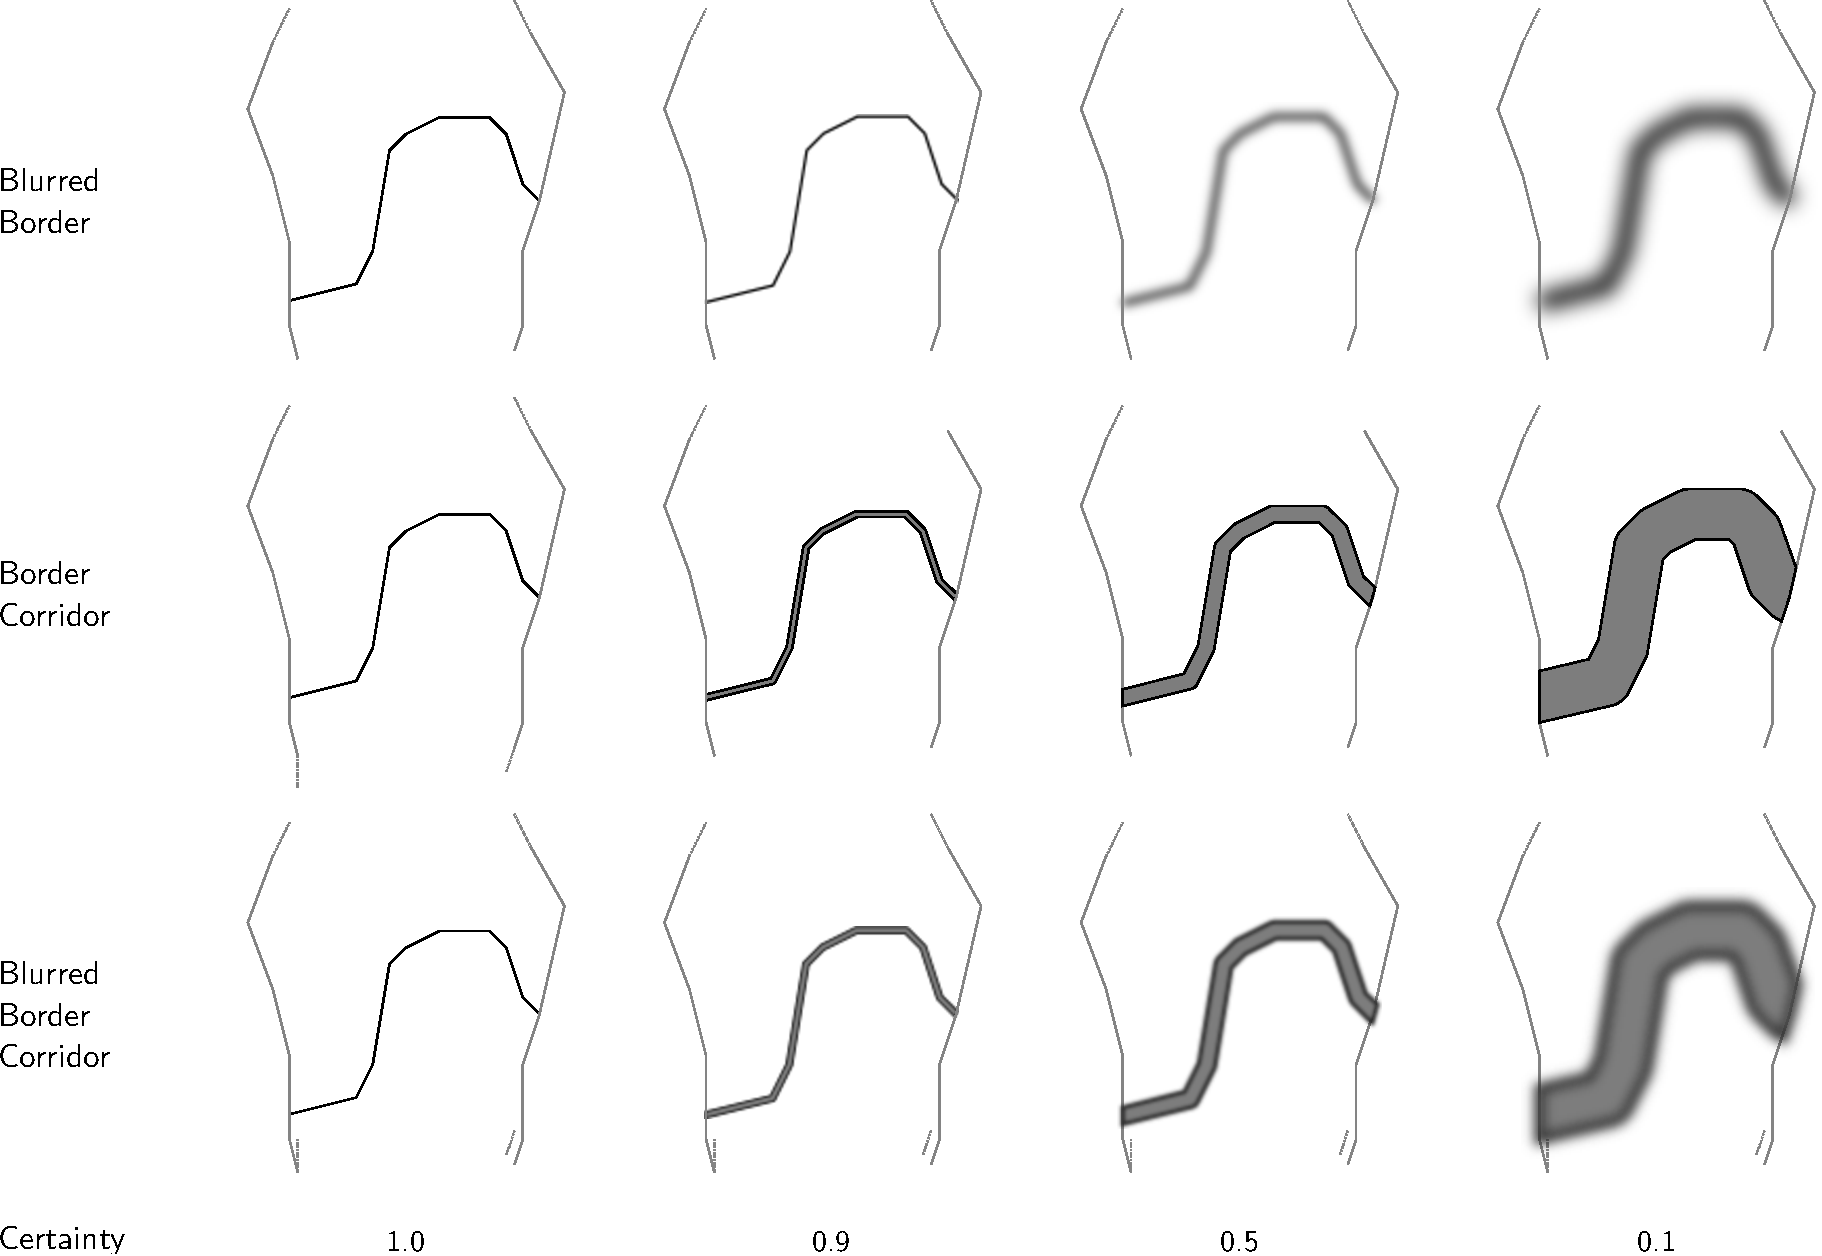
\includegraphics[width = 0.8\textwidth]{graphics/uncertainty/border}
  \caption{Three different methods to visualize uncertain courses of a border}
  \label{fig:uncertainty_border}
\end{figure}

Another advantage of the input of borderlines instead of territories is that once the model is further advanced, coastlines can be continuously changed according to an appropriate change model (see problem \ref{problem_general_coastlines}). This can be applied solely to the coastlines without affecting the interior borders.

A new border point automatically snaps to an existing border point, if the mouse position is close enough to it (an appropriate threshold might be $5~px$). This allows for a smooth workflow and is required to create closed polygons. In case the borderline is closed, it gets treated as a complete polygon and territory. When the user finished a territory by defining all surrounding polylines that create a closed ring, the polygon gets assembled. If a borderline meets another borderline at an interior node, the polyline gets split up into two parts so that each meeting point of borders is the start or end point of a polyline. This way integrity is maintained and each territory compounds of several polylines creating a set of closed polylines: a polypolygon.

\begin{figure}[H]
  \centering
  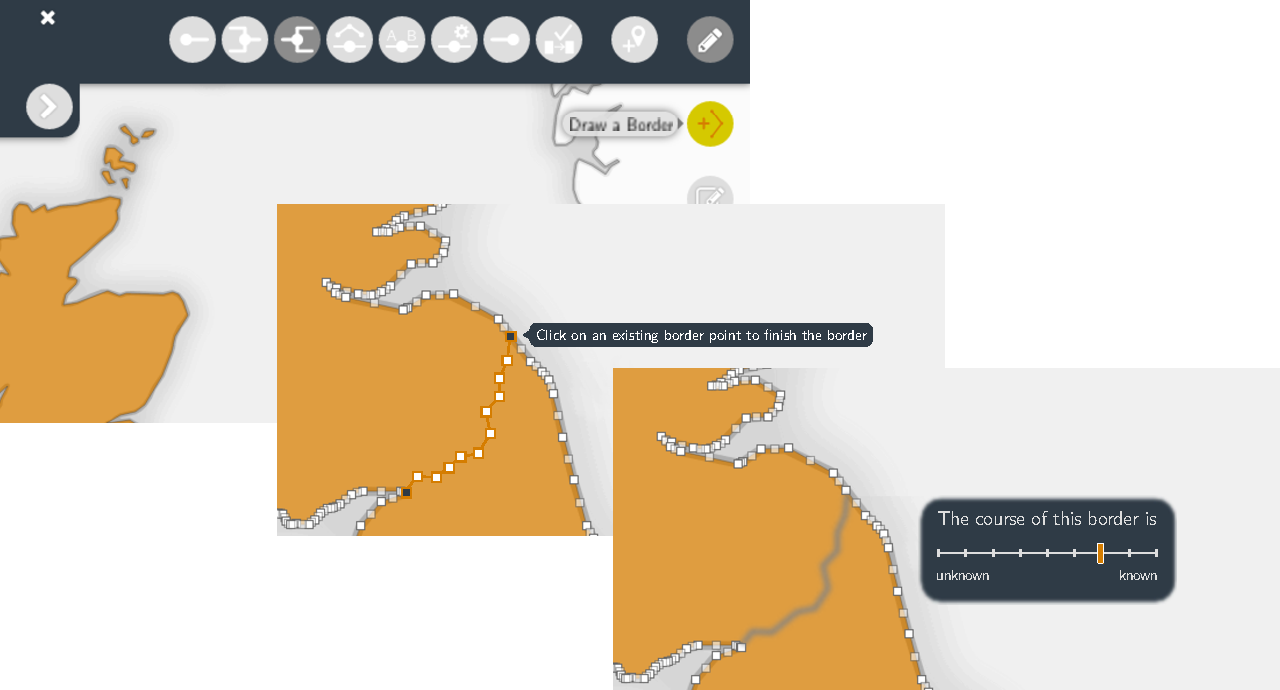
\includegraphics[width = 0.8\textwidth]{graphics/uncertainty/new_territory_tool}
  \caption{Drawing historical borders instead of full areas and definining a level of certainty.}
  \label{fig:uncertainty_new_territory_tool}
\end{figure}

If the created territory overlaps with an existing territory, its intersection will created a separate territory. In the next step, this territory can then be defined as a contested area or defined as a part of another area. If the step yields an empty territory that was claimed before, it can later be defined as a neutral zone or unclaimed land.

% paragraph set_new_territory (end)


\paragraph{Set New Name} % (fold)
\label{par:set_new_name}

When defining the name of an area, the user will get actual name suggestion. These result from a collection of current and historical countries from Wikipedia. That saves time for researching short and formal names of areas. In the long run, the system can be synchronized with Wikipedia or even be designed as an extension for Wikipedia articles about current or historical countries.

\begin{figure}[H]
  \centering
  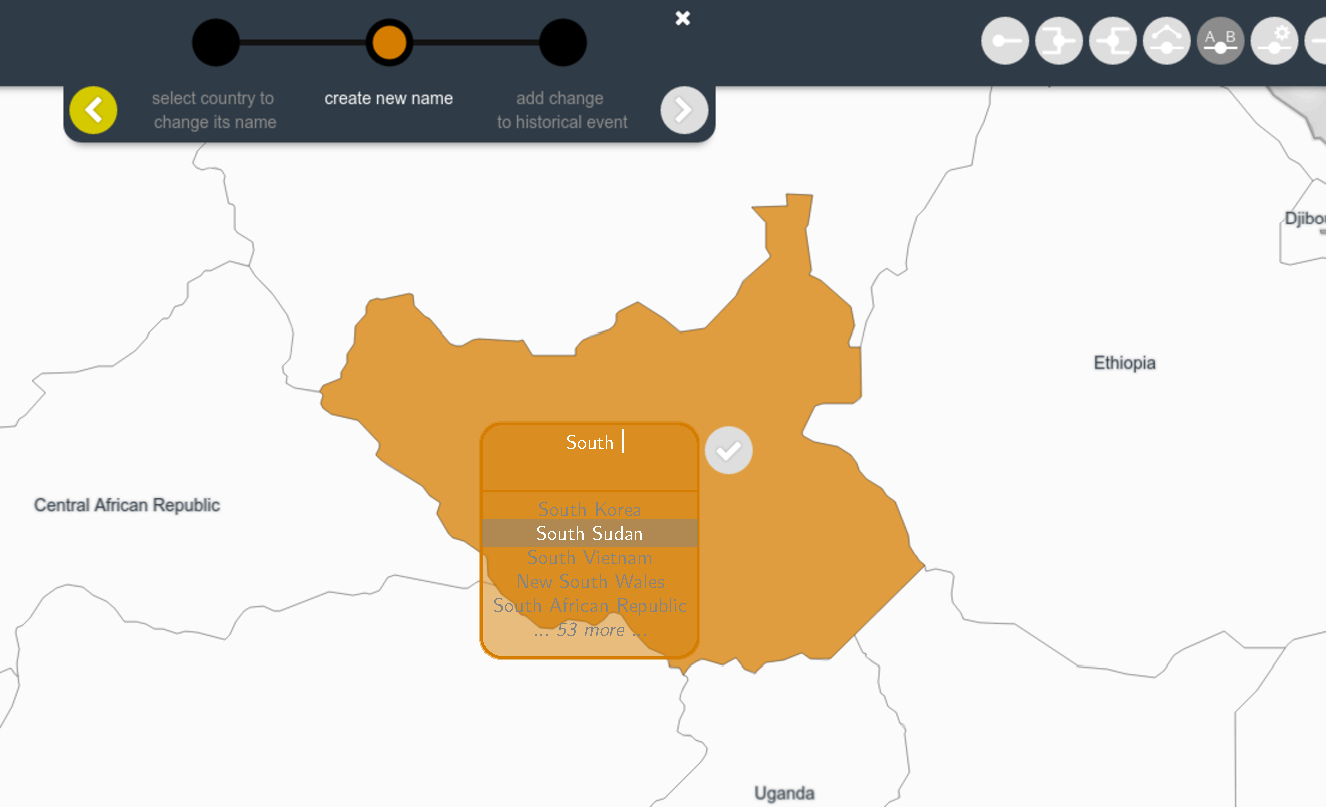
\includegraphics[width = 0.8\textwidth]{graphics/uncertainty/new_name_tool}
  \caption{Getting suggestions for the name name from Wikipedia.}
  \label{fig:uncertainty_new_name_tool}
\end{figure}

% paragraph set_new_name (end)

\paragraph{Set New Status} % (fold)
\label{par:set_new_status}

To treat special areas differently, a new step in the edit operation workflow gets defined. After the territory and the name of a new area are defined, a special status can be assigned to it:

\begin{enumerate}
  \item A \emph{fully sovereign country} is a political entity with full sovereignty over its territory and people and significant international recognition, e.g. Estonia.
  \item An \emph{unclaimed land} is a territory that is not claimed by any political entity, e.g. currently Antarctica.
  \item A \emph{neutral zone} is often a buffer zone between two conflicting countries, e.g. the UN Buffer Zone in Cyprus.
  \item A \emph{contested territory} is claimed by at least two different political entities of the same hierarchical level, e.g. the Kashmir region between India and Pakistan. It is also suitable for areas that have claimed independence from a sovereign country but are not yet regonized as such, making their whole territory contested, e.g. Nagorno-Karabakh (see figure \ref{fig:uncertainty_new_status_tool}).
  \item A territory can be a subordinate part of another country with a certain degree of autonomy ($\in [0..1]$). Fully subordinate parts of a country, like a US State or a German Bundesland have no autonomy ($0$). Autonomous countries within another country, like England to the United Kingdom or Greenland to Denmark, receive have certain a degree of autonomy ($\in ]0..1[$). Full autonomy ($1$) would mean the territory is a fully sovereign country and the value can therefore not be set in the options.
\end{enumerate}

\begin{figure}[ht]
  \centering
  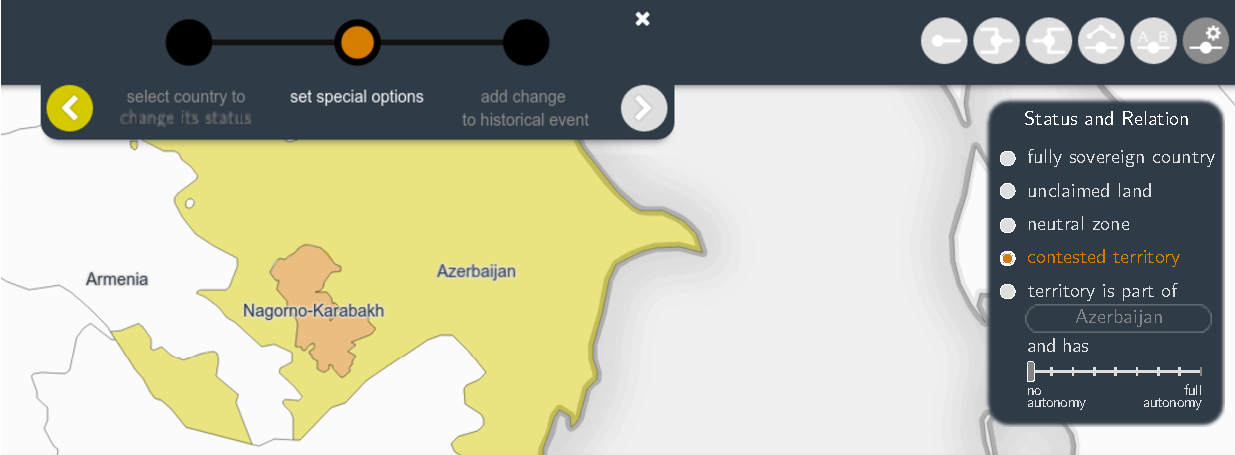
\includegraphics[width = 0.8\textwidth]{graphics/uncertainty/new_status_tool}
  \caption{Defining a special status or relationship to a territory.}
  \label{fig:uncertainty_new_status_tool}
\end{figure}

% paragraph set_new_status (end)


\paragraph{Add Historical Change} % (fold)
\label{par:add_historical_change}

The visualization of an Hivent gets split up into three parts:

\begin{enumerate}
  \item An information section storing important meta data of the event location, the dates (timespan in which the event happened), a description and the lin kto the wikipedia article (if given).
  \item A section storing all historical changes associated with that historical event. Each historical change is visualized and is assigned a date at which this event came into effect.
  \item A multimedia section stores images, videos, audio files and documents and their sources associated to the historical event.
\end{enumerate}

Similar to the extension of the area name step, also Hivent names can be chosen among a collection of Wikipedia articles describing historical events. Selecting a name from a wikipedia article automatically fills the information section and adds multimedia files from the wikipedia article. The historical change will automatically be entered in the section (see figure \ref{fig:uncertainty_new_hivent_box}). With this separation, different historical changes at different dates can be associated with one historical events, largely increasing the \texttt{Hivent} data model.

\begin{figure}[H]
  \centering
  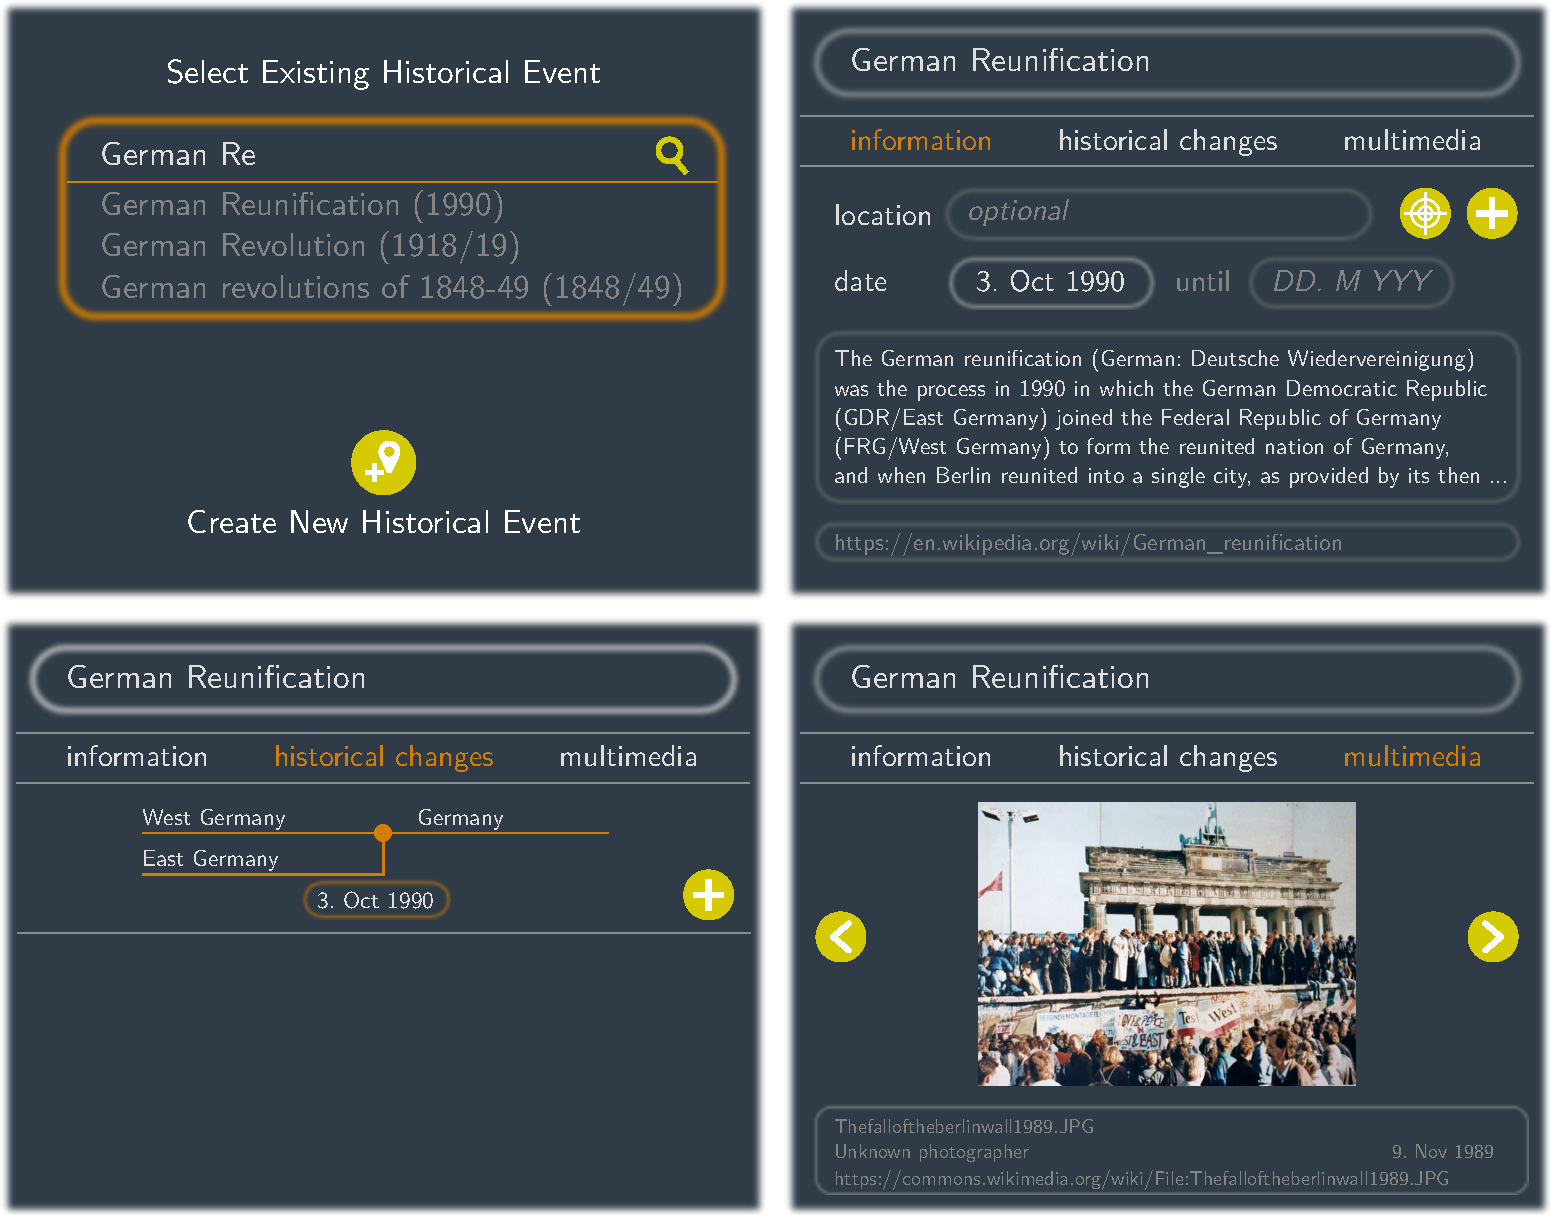
\includegraphics[width = 0.8\textwidth]{graphics/uncertainty/new_hivent_box}
  \caption{Creating a new Hivent and adding the newly created historical change.}
  \label{fig:uncertainty_new_hivent_box}
\end{figure}

% paragraph add_historical_change (end)



\paragraph{New Area Recognition} % (fold)
\label{par:new_area_recognition}

One new operation is to add the recognition of one country by another country. That is simply performed by selecting two areas on the map, whereas the first area recognized the second area. This is an historical change that can afterwards be attached to an Hivent.

\begin{figure}[H]
  \centering
  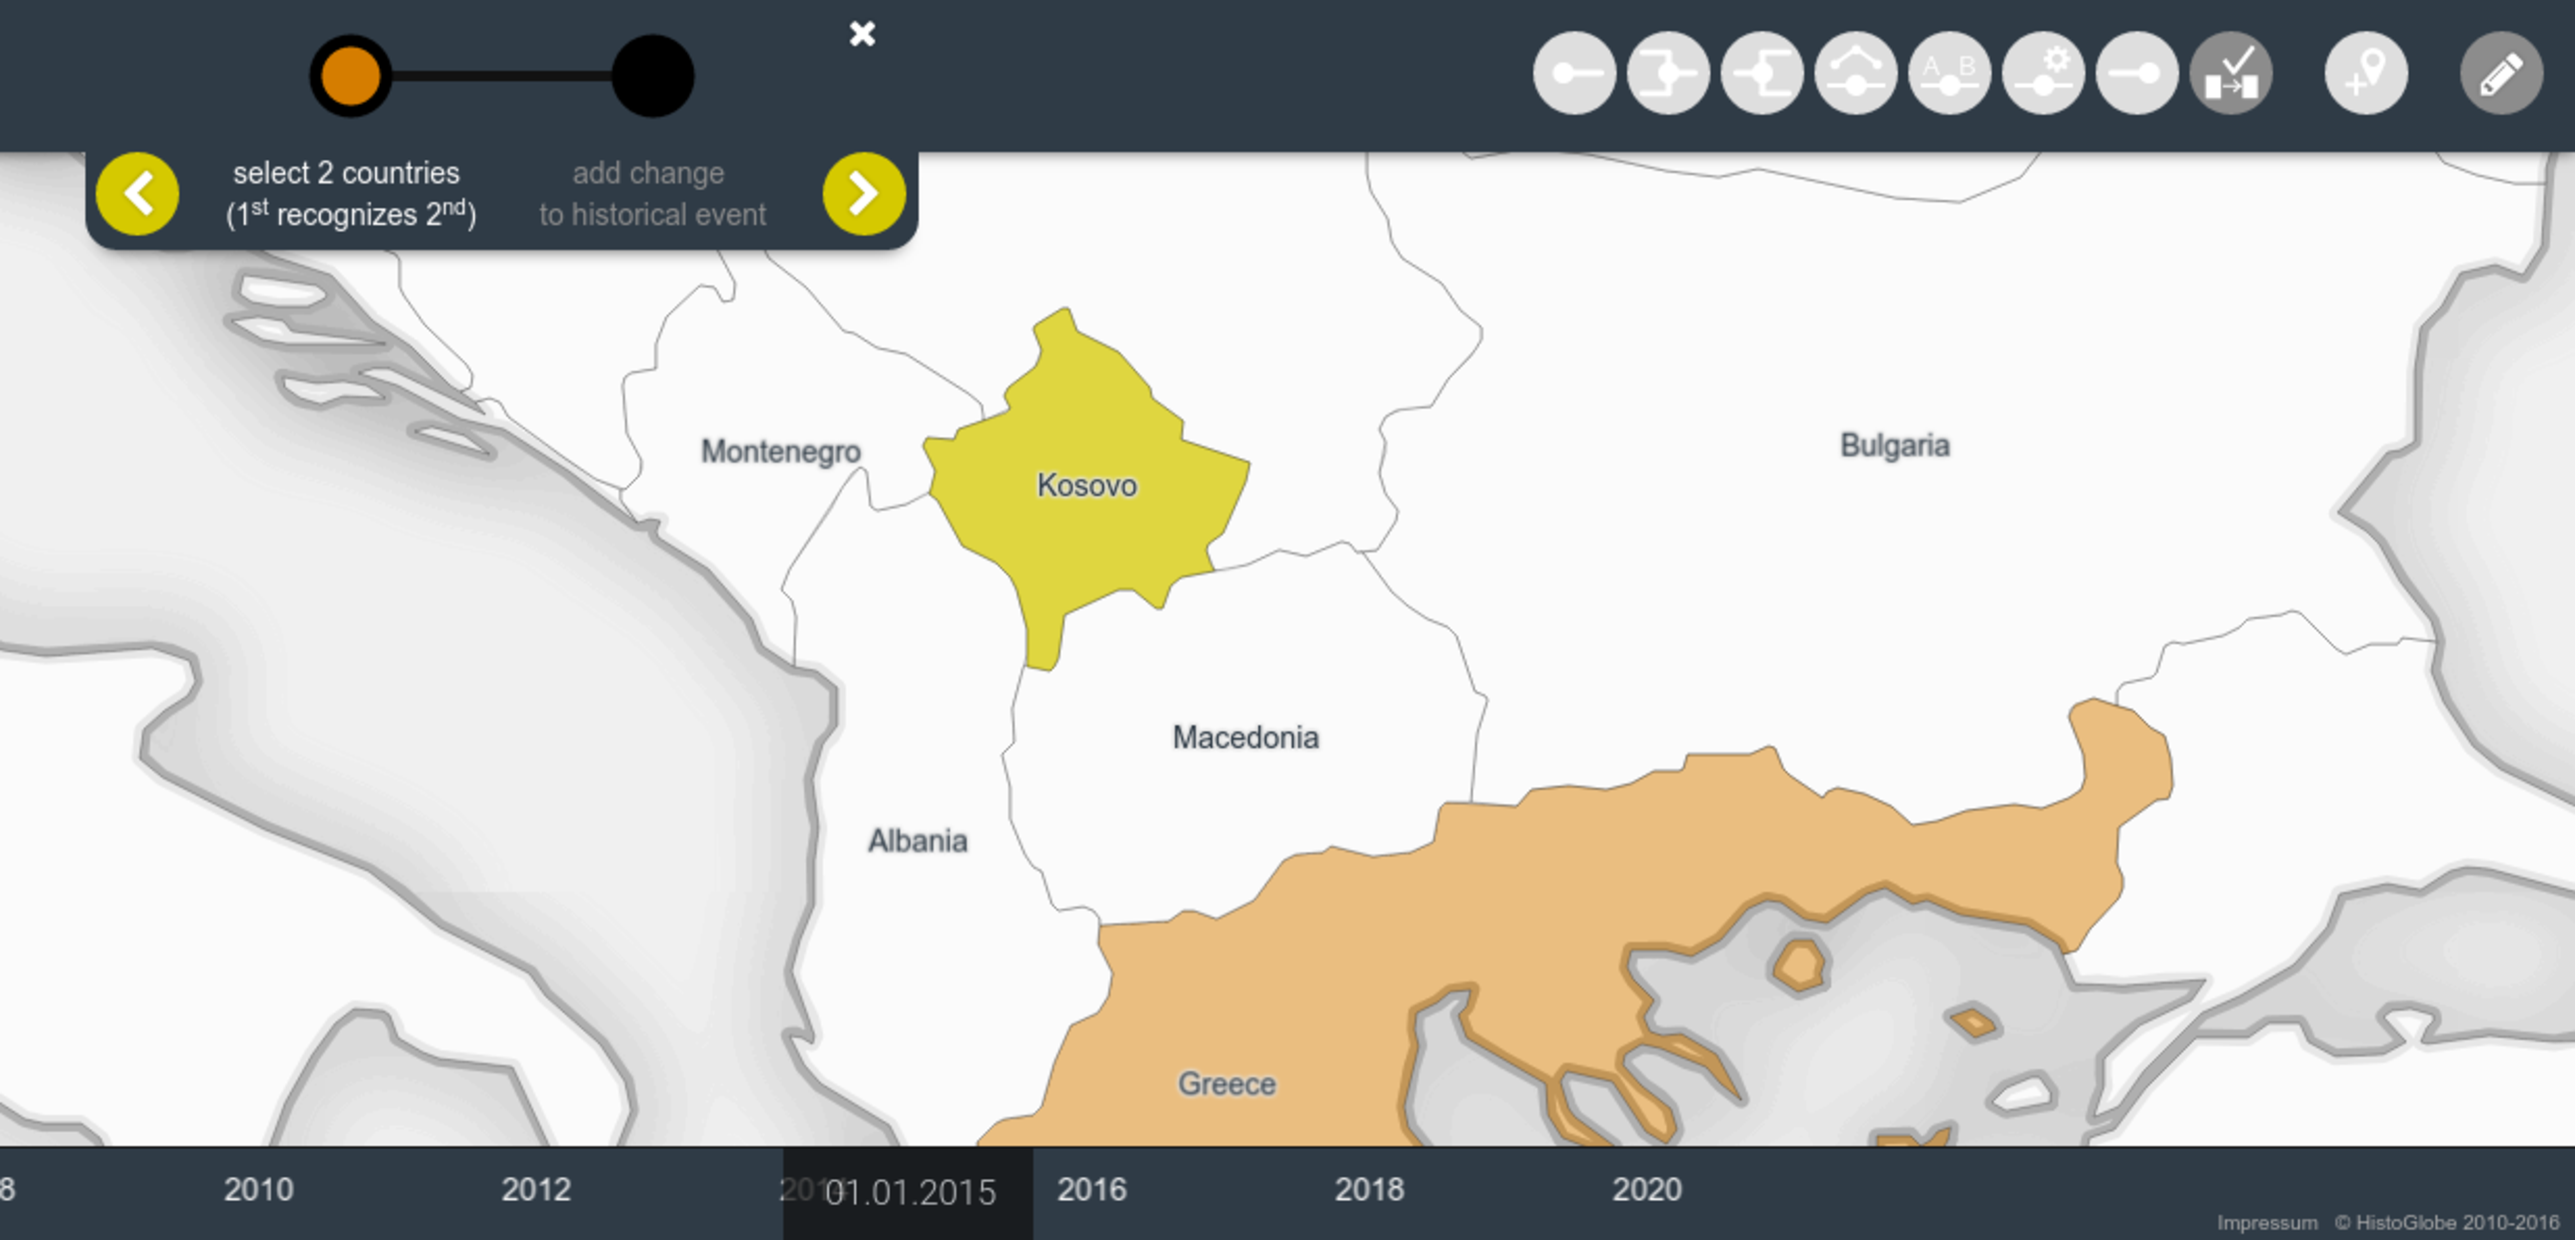
\includegraphics[width = 0.8\textwidth]{graphics/uncertainty/operation_REC}
  \caption{New edit operation: Recognition -- sets up the recognition of one area to another.}
  \label{fig:uncertainty_operation_REC}
\end{figure}


% paragraph new_area_recognition (end)

\paragraph{Multi-language support} % (fold)
\label{par:multi_language_support}

In order to support different languages, a language selection is placed on the bottom right corner of the interface, on the timeline (see figure \ref{fig:multi_language}). This changes the language of the whole interface and loads the translations of the area names and the Hivent names, locations and descriptions in the newly created language. If a term is not defined in the language, the fallback language (English) is used instead.

\begin{figure}[H]
  \centering
  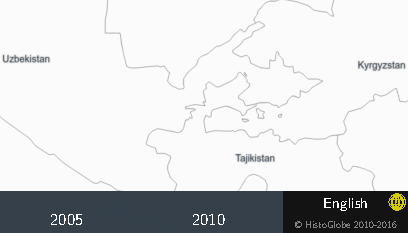
\includegraphics[width = 0.45\textwidth]{graphics/uncertainty/multi_language}
  \caption{Changing the language in the user interface.}
  \label{fig:multi_language}
\end{figure}


% paragraph multi_language_support (end)


% subsection extension_of_the_edit_mode (end)

% ------------------------------------------------------------------------------
\subsection{Extension of the Data Model} % (fold)
\label{sub:extension_of_the_data_model}

To account for the changes in the interface, also the data model has to be adapted. The main changes to the original data model developed in section \ref{cha:development} are:
% TODO: real section of original data model

\begin{enumerate}
  \item Creation of a \texttt{Multilang} entity to store a name of an Hivent, its location or an Area name in different languages.
  \item Outsourcing of the \texttt{HiventLocation} into an own entity to identify a location with a name and a geospatial reference.
  \item Creation of a \texttt{Multimedia} entity to manage multimedia files associated to an Hivent.
  \item Attachment of a date to an \texttt{HistoricalChange}.
  \item Inclusion of the \texttt{formal\_name} into the \texttt{Area} model to emphasize it as the identifier of an area.
  \item Creation of an \texttt{AreaBorder} with a \texttt{borderline}. A set of \texttt{AreaBorders} create one \texttt{AreaTerritory} which is associated to the Area. Each change of an \texttt{AreaBorder} creates one or two new \texttt{AreaTerritory}/ies.
  \item Creation of an \texttt{AreaStatus} an an \texttt{AreaRelation} to account for special status of an area alone or in relation to another area with a certain level of autonomy.
  \item Creation of an \texttt{AreaRecognition} to account for international recognition of one area to another one.
  \item Adaption of the \texttt{AreaChange} entity to model a change of each possible property of an area.
\end{enumerate}


\begin{figure}[ht]
  \centering
  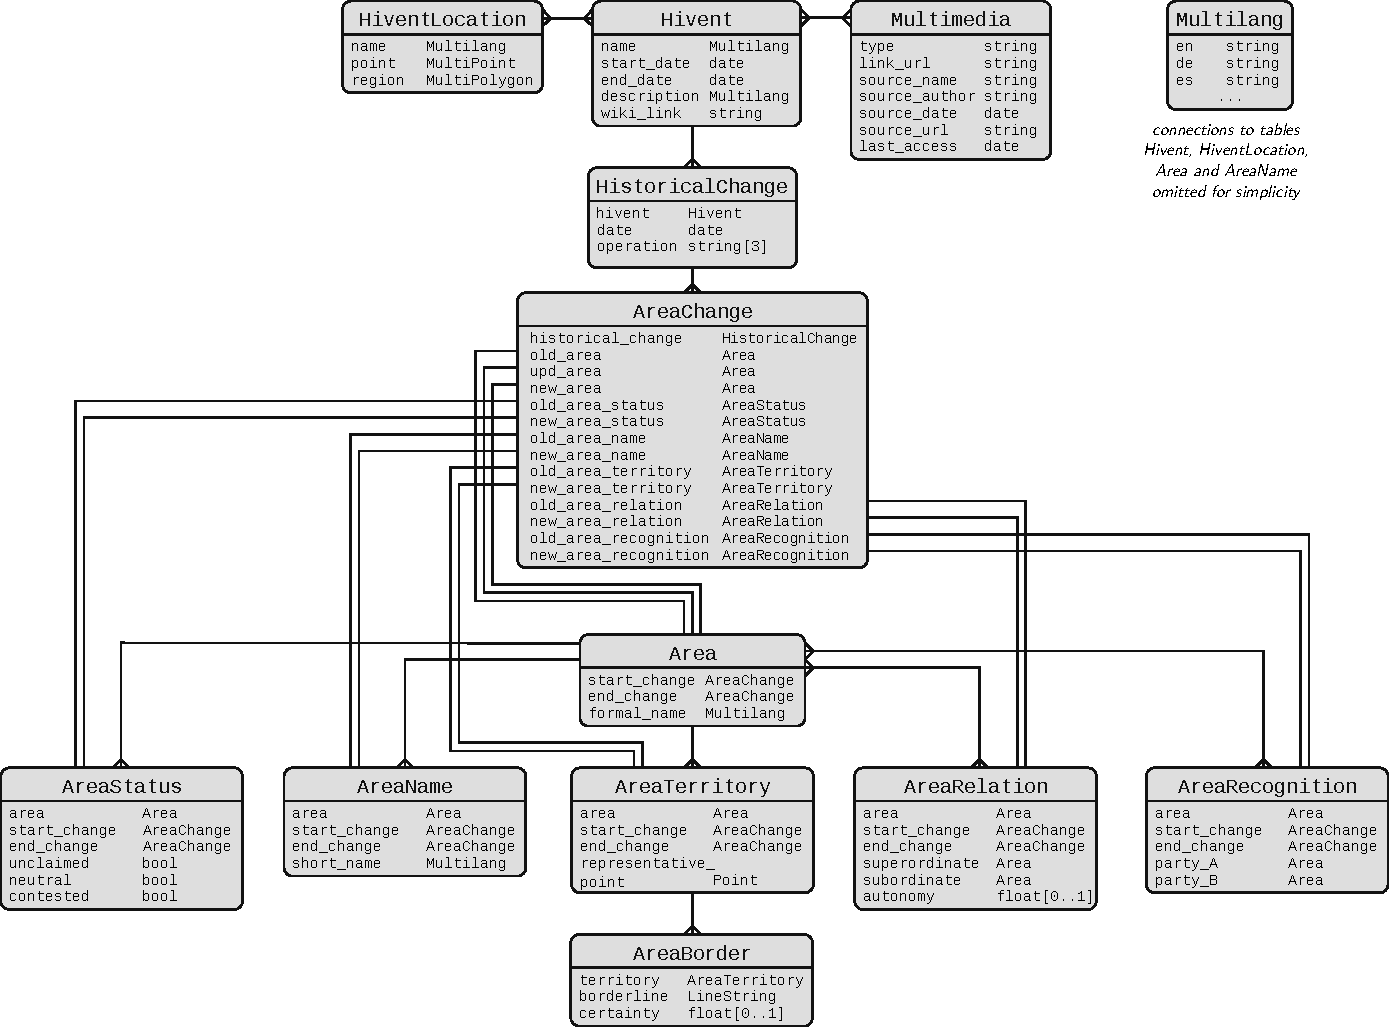
\includegraphics[width = 0.8\textwidth]{graphics/uncertainty/new_data_model}
  \caption{The new data model to support the developed approaches regarding uncertainty}
  \label{fig:new_data_model}
\end{figure}

% subsection extension_of_the_data_model (end)

% section solution_approaches (end)


% ==============================================================================

% chapter uncertainty (end)